\section{The original experiment and what it measured}\label{sec:original}

\subsection{Setup as run}

The network has four convolution blocks (64, 128, 256, and 512 channels; each a 3$\times$3 convolution, batch normalization~\cite{ioffe2015batch}, ReLU, and 2$\times$2 max pooling), a spatial attention layer after the first block, global average pooling, and a linear layer to a \N{emb}-dimensional embedding: \N{params} parameters, \N{params_att} of them in the attention layer. It was trained once, on \N{orig_train_images} CelebA-HQ images at 256$\times$256 drawn without a seed (the list was not saved), for \N{orig_epochs} epochs with batch size \N{orig_batch}, Adam~\cite{kingma2015adam} at a learning rate of \N{orig_lr}, and a triplet loss with margin \N{orig_margin}. Each triplet's anchor was an image, its positive the same image with a centered black square covering \N{orig_occ_lo} to \N{orig_occ_hi}\% of its area, and its negative a random other image. Inputs were scaled to $[0,1]$ without normalization.

The test drew $N$ images (a new unseeded sample per run). The gallery held the clean images, and each probe was one of them with a centered black square covering a share of the 256$\times$256 frame, at 21 levels from 0 to 100\% in steps of 5\%. A probe counted as correct if its nearest gallery embedding, by Euclidean distance, was its own clean image. The six pretrained models ran through DeepFace \N{deepface_v}~\cite{serengil2020lightface,deepface} with its default detector, OpenCV's Haar cascade~\cite{viola2001rapid,bradski2000opencv}, and \texttt{enforce\_detection} off, matched by Euclidean distance on unnormalized embeddings. The reported runs are one each at $N=50$, 100, 200, and 500 (Google Colab, A100 runtime), and three on copies of the $N=50$, 100, and 200 samples with backgrounds removed; the other files in \texttt{results/\allowbreak original/} (two runs in steps of 1\%, earlier background-removed runs, and pipeline tests) are not used here, except one background-removed $N=50$ run that repeats a reported one (Section~\ref{sec:bg}). The results are in Table~\ref{tab:original}, Table~\ref{tab:lead}, and Fig.~\ref{fig:original}.

\begin{table}[t]
\caption{Original $N=100$ run: share of probes matched to their own clean image (\%), with nearest neighbor on raw pixels of the same images. Occlusion is the square's share of the 256-pixel frame; the 35, 45, 55, and 65 to 95\% rows are left out. One unseeded run. Cust.\ = the project's model; VGG = VGG-Face; FN = FaceNet; FN512 = DeepFace's 512-dimensional FaceNet; OF = OpenFace; AF = DeepFace's ArcFace; SF = SFace.}
\label{tab:original}
\centering\small
\setlength{\tabcolsep}{4pt}
% Generated by make_numbers.py. Do not edit.
\begin{tabular}{@{}rrrrrrrrr@{}}
\toprule
Occ. & Cust. & VGG & FN & FN512 & OF & AF & SF & Pixels \\
\midrule
0\% & 100 & 100 & 100 & 100 & 100 & 100 & 100 & 100 \\
5\% & 100 & 72 & 5 & 34 & 4 & 3 & 16 & 100 \\
10\% & 99 & 13 & 1 & 1 & 3 & 1 & 2 & 100 \\
15\% & 96 & 3 & 2 & 2 & 3 & 0 & 2 & 95 \\
20\% & 90 & 2 & 2 & 2 & 6 & 0 & 2 & 76 \\
25\% & 81 & 2 & 2 & 1 & 2 & 1 & 1 & 68 \\
30\% & 73 & 2 & 2 & 1 & 3 & 1 & 1 & 54 \\
40\% & 50 & 1 & 2 & 1 & 2 & 1 & 0 & 30 \\
50\% & 31 & 1 & 1 & 1 & 2 & 1 & 1 & 16 \\
60\% & 18 & 1 & 1 & 1 & 1 & 0 & 2 & 11 \\
100\% & 1 & 1 & 1 & 1 & 1 & 1 & 1 & 1 \\
\bottomrule
\end{tabular}

\end{table}

\begin{figure*}[t]
\centering
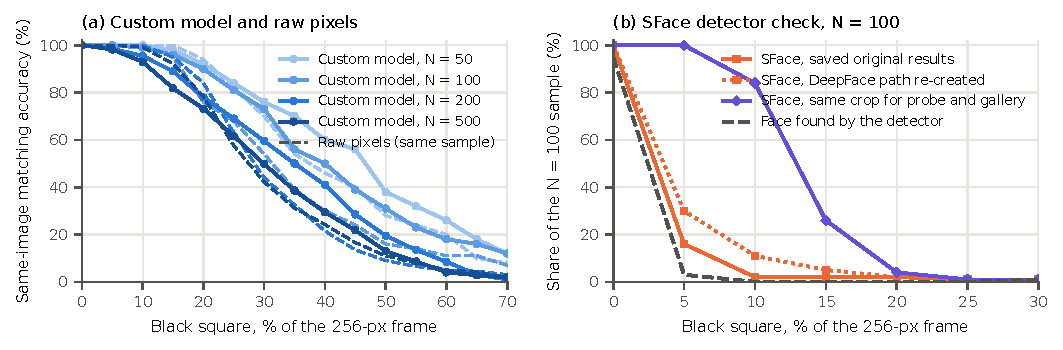
\includegraphics[width=\textwidth]{figures/fig_original.pdf}
\caption{The original runs on their own axis, the black square's share of the 256-pixel frame (not comparable with the crop coverage of Figs.~\ref{fig:squares}, \ref{fig:other}, and~\ref{fig:gap}a). Panel (a) stops at 70\% and panel (b) at 30\%. (a) The project's model at each $N$ (solid) and nearest neighbor on raw pixels of the same sample (dashed, same shade); each $N$ is one unseeded sample and run. (b) For SFace on the $N=100$ sample: the saved original results, the CPU re-creation of DeepFace's detector path, SFace with the same face crop for probe and gallery, and the share of images in which the detector finds a face. Panel (b) uses the original's Euclidean matching on unnormalized embeddings throughout.}
\label{fig:original}
\end{figure*}

\subsection{Image matching, not identification}

Each probe is its own gallery image with a square drawn on it, and nothing tests a second photo of the same person, so these results measure how well an occluded image is matched to its clean copy. That task is easy at low occlusion: nearest neighbor on raw pixels, with no learning, matches \N{px_50_10}, \N{px_100_10}, and \N{px_200_10}\% of images at 10\% occlusion for $N=50$, 100, and 200, \N{px_500_10}\% at $N=500$, and \N{px_100_20}\% at 20\% for $N=100$ (Table~\ref{tab:original}). At 100\% occlusion, every model and raw pixels score \N{o_100_cu_100}\%, chance for $N=100$. The original report's ``face recognition'' results are results on this matching task.

\subsection{The pretrained models' collapse: the detector, for SFace}

The pretrained models fall from 100\% clean to \N{o_100_pre_10_lo} to \N{o_100_pre_10_hi}\% at 10\% occlusion (Table~\ref{tab:original}), while raw pixels still match every image. The original runs saved no detection results, so the detector's part was re-created on a CPU for SFace alone, with OpenCV's Haar cascade at DeepFace \N{deepface_v}'s settings, without DeepFace's eye alignment, and with the original's Euclidean matching on unnormalized SFace embeddings. The cascade finds a face in \N{det_found_00} of the 100 clean images, \N{det_found_05} at 5\%, and \N{det_found_10} at 10\%. When it finds none, the whole frame is embedded and compared with a gallery of mostly face crops, and \N{det_one_10}\% of the probes at 10\% land on one and the same gallery image. With the same face crop for probe and gallery, SFace matches \N{det_same_05}\% at 5\% and \N{det_same_10}\% at 10\%, against \N{det_saved_05}\% and \N{det_saved_10}\% in the saved results (Fig.~\ref{fig:original}b), so most of SFace's collapse at 5 to 10\% is the detector. The re-creation is approximate: its version of DeepFace's path gives \N{det_path_05}\% and \N{det_path_10}\%, not the saved \N{det_saved_05}\% and \N{det_saved_10}\%. Only SFace was rerun, and VGG-Face's \N{o_100_vgg_05}\% at 5\% shows that the effect differs by model, so for the other five models, the detector is the likely cause, not a measured one.

From 15\% on, the square covers much of the face itself: a median \N{cov_15}\% of the detected face box (median side \N{face_box} pixels) at 15\% and \N{cov_50}\% at 50\%. There, SFace fails with either crop under the original's matching: \N{det_same_15} to \N{det_whole_15}\% at 15\% and \N{det_same_20} to \N{det_whole_20}\% at 20\%, for the same face crop and for whole frames on both sides.

\subsection{The project's model against raw pixels}

The project's model matches \N{o_100_cu_10}, \N{o_100_cu_20}, \N{o_100_cu_30}, and \N{o_100_cu_50}\% at 10, 20, 30, and 50\% occlusion for $N=100$. Its lead over raw pixels (Table~\ref{tab:lead}) is at most one image through 15\% occlusion, starts at 20 to 25\%, and depends on the sample. Through 20\%, raw pixels match or beat it at $N=50$, 200, and 500 (at $N=500$, by \N{lead_500_10_abs} points at 10\% and \N{lead_500_15_abs} at 15\%); of the four original samples, only $N=100$ shows a lead at 20\% (\N{lead_100_20}). At 30\%, the lead is \N{lead_50_30}, \N{lead_100_30}, \N{lead_200_30}, and \N{lead_500_30} points for $N=50$, 100, 200, and 500, and at $N=500$, it is never more than \N{lead_500_max} points. The study in Section~\ref{sec:design} adds a fifth sample under the same protocol, \N{n_gallery} seeded frames, with raw pixels of the frame downsampled to \N{frame_small}$\times$\N{frame_small}: pixels lead by \N{lead_study_05_abs} to \N{lead_study_10_abs} points at 5 to 15\%, and the model leads by \N{lead_study_50_abs} to \N{lead_study_30_abs} points from 20 to 50\%. About 1 in \N{orig_overlap_share} of those frames was probably among the model's training images (an estimate: \N{orig_train_images} of \N{n_label_images}). The four original samples are unseeded single runs of one trained model, so their run-to-run variation is unknown, and no interval here covers it.

Past about 30\%, the square covers most of the face box (a median \N{cov_30}\% of the box at 30\%, \N{cov_40}\% at 40\%), yet the model still matches \N{o_100_cu_40}\% at 40\% for $N=100$. That accuracy likely rests mostly on what lies outside the face box, such as hair, background, and clothes; no run tested this directly.

\begin{table}[t]
\caption{The project's model minus raw pixels, in percentage points, under the original protocol. Columns $N=50$ to 500 are the original runs (one unseeded sample each); ``Study'' is the saved model on the study's \N{n_gallery} seeded gallery frames, against raw frame pixels downsampled to \N{frame_small}$\times$\N{frame_small}. Occlusion is the square's share of the frame.}
\label{tab:lead}
\centering\small
% Generated by make_numbers.py. Do not edit.
\begin{tabular}{@{}rrrrrr@{}}
\toprule
Occ. & $N=50$ & $N=100$ & $N=200$ & $N=500$ & Study \\
\midrule
5\% & 0 & 0 & $-$1.5 & $-$1.8 & $-$5.4 \\
10\% & 0 & $-$1 & $-$4.5 & $-$6.2 & $-$14.2 \\
15\% & $-$2 & +1 & $-$6 & $-$10.4 & $-$11.4 \\
20\% & $-$2 & +14 & $-$6 & $-$5.0 & +2.7 \\
25\% & +2 & +13 & +6 & +4.0 & +6.4 \\
30\% & +6 & +19 & +15.5 & +7.6 & +9.7 \\
35\% & +16 & +17 & +17.5 & +7.4 & +8.6 \\
40\% & +14 & +20 & +19.5 & +5.2 & +6.7 \\
50\% & +10 & +15 & +10.5 & +2.0 & +2.2 \\
\bottomrule
\end{tabular}

\end{table}

The saved model reproduces its results. Rerun on a CPU from the saved weights (a release asset of this repository) and samples (not in it), it differs from the result files by at most three images at any level: \N{rerun_n50_max} points at $N=50$, \N{rerun_n100_max} at $N=100$, and \N{rerun_n200_max} at $N=200$. Among the original run folders, also not in the repository, those of $N=50$ and $N=200$ hold copies of the weights with one hash; for $N=100$, the evidence is indirect (the code loads the saved file, which predates the run, and the rerun reproduces it), and $N=500$ has neither a copy nor a rerun.

\subsection{Background removal}\label{sec:bg}

Backgrounds were replaced with white by rembg~\cite{rembg} (U$^2$-Net~\cite{qin2020u2net}), and each of these runs fine-tuned the saved model for \N{orig_epochs} more epochs on its own background-removed test images. At $N=100$, the project's model fell from \N{o_100_cu_20} to \N{o_nobg100_cu_20}\% at 20\% occlusion and from \N{o_100_cu_30} to \N{o_nobg100_cu_30}\% at 30\%. The cause is unclear. Raw pixels do better without the background (\N{px_nobg100_20}\% at 20\%, against \N{px_100_20}\%), so the images can still be matched (whether the model lost cues it relied on was not tested); the saved model before fine-tuning scores \N{master_nobg100_20}\% at 20\% on the same background-removed images, above the fine-tuned \N{o_nobg100_cu_20}\%; and the same fine-tuning code, on the same 50 images from the same saved weights, gave \N{o_nobg50a_cu_20}\% in one run and \N{o_nobg50b_cu_20}\% in another at 20\%. The drop is real for these single runs and is not explained by images that can no longer be matched, but unseeded fine-tuning on 50 images (the only size repeated) varied too much from run to run to say more.
